\textbf{Note: }\textit{The majority of the work presented in this chapter was published in two independent pieces of work. All work relating to the globular targets was published by \textcite{Simkovic2016-wk}, and a great majority of work relating to the transmembrane targets by \textcite{Thomas2017-sh}. As such, this chapter consists of extracts from both publications with additional information where appropriate. Text duplicated from either publication was written by Felix Simkovic, all other elements were adapted.}

\section{Introduction}
The introduction of residue-residue contacts as distance restraints in \textit{ab initio} protein structure prediction has proven to be a highly successful approach to limiting the conformation search space thereby enabling successful fold prediction of larger and more \textbeta-rich protein structures \cite[e.g.,][]{Marks2011-os,Michel2014-eg,Kosciolek2014-bt,Ovchinnikov2015-tn,Ovchinnikov2016-jj,Michel2017-xh,De_Oliveira2017-sg,Ovchinnikov2017-nd,Wang2017-rx}. In AMPLE, these two domains are the major limitation for a more successful approach \cite{Bibby2012-lm}. This typically results in user success being limited to small globular and primarily \textalpha-helical folds, or time- and resource-demanding attempts most likely going to be unsuccessful for larger targets

With the advent of contact information, is has thus become essential to identify the extend to which this invaluable bit of information is going to help AMPLE users in the future.

\section{Materials \& Methods}
\subsection{Target selection}
In this study, targets from the ORIGINAL and TRANSMEMBRANE datasets were used. This resulted in a final set of 21 globular and 17 transmembrain protein targets. For details in how the targets were selected refer to \cref{sec:methods_dataset_original,sec:methods_dataset_transmembrane}, and for details on each target refer to \cref{table:appendix_dataset_transmembrane,table:appendix_dataset_original}.

\subsection{Contact prediction} \label{sec:ample_proof_conpred}
For all globular targets, one contact map was predicted with the fully automated metapredictor PCONSC2 v1.0 \cite{Skwark2014-qp}. In summary, four \gls{msa}s were generated with JACKHMMER v3.1b2 \cite{Johnson2010-uz} against the \texttt{uniref100} v2015-10 database and HHBLITS v2.0.15 \cite{Remmert2011-kt} against the \texttt{uniprot20} v2013-03 database \cite{Bateman2017-pb} at E-value cutoffs of 10\textsuperscript{-40}, 10\textsuperscript{-10}, 10\textsuperscript{-4} and 1. Each \gls{msa} was analysed with PSICOV v2.13b3 \cite{Jones2012-ks} and PLMDCA v2 \cite{Ekeberg2014-kf} to produce 16 individual contact predictions. All 16 predictions and per-target PSIPRED v3 \cite{Jones1999-ed} secondary structure prediction, NETSURFP v1.0 \cite{Petersen2009-wy} solvent accessibility information and HHBLITS v2.0.15 \cite{Remmert2011-kt} sequence profile were provided to the PCONSC2 deep learning algorithm \cite{Skwark2014-qp} to identify protein-like contact patterns. The latter produced a final contact map for each target sequence.

An additional contact map for \textbeta-structure containing targets was predicted using CCMPRED v0.3 \cite{Seemayer2014-zp} and reduced to \textbeta-sheet contact pairs using the CCMPRED-specific filtering protocol BBCONTACTS v1.0 \cite{Andreani2015-qn}. Each \gls{msa} for CCMPRED contact prediction was obtained using HHBLITS v2.0.15 \cite{Remmert2011-kt}. This entailed two sequence search iterations with an E-value cutoff of 10\textsuperscript{-3} against the \texttt{uniprot20} v2013-03 database \cite{Bateman2017-pb} and filtering to 90\% sequence identity using HHFILTER v2.0.15 \cite{Remmert2011-kt} to reduce sequence redundancy in the \gls{msa}. Besides the contact matrix as input, BBCONTACTS requires a secondary structure prediction and an estimate of the \gls{msa} diversity. The secondary structure prediction was taken from the PCONSC2 step whilst the diversity factor was calculated using \cref{eq:methods_alndiversity}.

For each transmembrane protein target, a \gls{msa} was generated using HHBLITS v2.0.16 \cite{Remmert2011-kt} against \texttt{uniprot20} v2016-02 database \cite{Bateman2017-pb}. Contact predictions for each transmembrane target were obtained using the metapredictor METAPSICOV v1.04 \cite{Jones2015-vq}, which in turn used the contact prediction algorithms CCMPRED v0.3.2 \cite{Seemayer2014-zp}, FREECONTACT v1.0.21 \cite{Kajan2014-bx} and PSICOV v2.1b3 \cite{Jones2012-ks}. Additionally, a set of contacts was also generated using the MEMBRAIN server v2015-03-15 \cite{Yang2013-bf}.

\subsection{Contact-to-restraint conversion} \label{sec:bbcontacts_addition}
For all targets, the predicted contact maps were converted to ROSETTA restraints to guide \textit{ab initio} structure prediction. The FADE energy function was used to introduce a restraint in ROSETTA's folding protocol. The implementation described by \textcite{Michel2014-eg} was used, which defined a contact to be formed during folding if the participating C\textbeta\ atoms (C\textalpha\ in case of glycine) were within 9\AA\ of one another. The top-$L$ ($L$ corresponds to the number of residues in the target sequence) contact pairs were converted to ROSETTA restraints, and if satisfied a ``squared-well'' bonus of -15.00 added to the energy function.

Additionally to above, all \textbeta-containing targets were subjected to a further conversion step in a separate condition. The approach of adding BBCONTACTS restraints to a previous prediction is outlined in \cref{sec:methods_bbcontacts_addition}.

\subsection{\textit{Ab initio} structure prediction}
Fragments for all targets were selected using the \texttt{make\_fragments.pl} script shipped with ROSETTA. To ensure no homologous fragments were included in the fragment libraries, the \texttt{-nohoms} flag was set. Each target's secondary structure prediction was provided to the fragment picker using the \texttt{-psipredfile} argument. The fragment libraries, contact restraints and secondary structure prediction were subjected to the ROSETTA \texttt{AbinitioRelax} protocol \cite{Rohl2004-dj} to predict 1,000 decoys per target. ROSETTA options were chosen according to the default protocol in AMPLE v1.0 \cite{Bibby2012-lm}. ROSETTA v2015.05.57576 was used for globular targets and v2015.22.57859 for transmembrane ones for all ROSETTA-related protocols.
%
\subsection{Molecular Replacement in AMPLE}
All generated decoys were subjected to AMPLE v1.0 \cite{Bibby2012-lm} for ensemble search model generation. 

All transmembrane protein targets were processing using AMPLE's default parameters. \Gls{mr} trials were performed with software versions shipped in CCP4 v6.5.13 \cite{Winn2011-xe}, with the exception of SHELXE v2014/14 \cite{Thorn2013-le} and ARP/wARP v7.5 \cite{Cohen2007-wg}.

All globular protein targets were subjected to AMPLE with two deviations from the default parameters. The \texttt{-use\_scwrl} was set to subject all decoys to side-chain remodelling using SCWRL4 \cite{Krivov2009-ex}. Furthermore, the number of clusters to trial was set increased from one to three via the \texttt{-num\_clusters}parameter. All \gls{mr} trials were performed with the version of software shipped with CCP4 v6.5.15 \cite{Winn2011-xe}.

All \gls{mr} solutions were assessed for success using the criteria described in \cref{sec:methods_mr_success}.

\section{Results}
In this study, the application of residue-residue contact predictions to \textit{ab initio} protein structure prediction and subsequently \gls{mr} was investigated. This proof-of-concept work is based on two datasets covering a range of globular and transmembrane protein targets. At the time of conducting this study, state-of-the-art contact prediction algorithms were applied to obtain the best possible contact predictions to identify the extend of pushing the boundaries previously incurred in AMPLE studies \cite{Bibby2012-lm}.

\subsection{Residue-residue contact prediction}
Accurate coevolution-based residue-residue contact prediction highly depends on the availability of many divergent homologous sequences. As such, it is important to validate that the selected targets in this study satisfy such requirement.

The depth of \gls{msa}s obtained for each target sequence suggests that sufficient numbers of divergent homologous sequences are available. Across all globular targets, the minimum alignment depth is obtained for Galectin-3 domain (\gls{pdb} ID: 1kjl) with 679 effective sequences and the maximum for G-protein Arf6-GDP (\gls{pdb} ID: 1e0s) with 1,897 effective sequences (\cref{fig:ample_proof_globpreccomp}). The median alignment depth for all globular targets is over 1,000, which is beyond the often suggested threshold of 200 sequences \cite{Simkovic2017-xs}. The \gls{msa}s for all transmembrane protein targets also surpass this threshold comfortably. The median alignment depth is much higher than for globular targets with 1,878 sequences (\cref{fig:ample_proof_tmpreccomp}). The minimum, which was obtained for Sensory rhodopsin II (\gls{pdb} ID: 1gu8), is 692 sequences and the maximum for the sequence of Rhomboid protease GLPG (\gls{pdb} ID: 2xov) is 6,583.

\begin{figure}[H]
    \centering
    \begin{subfigure}[b]{\textwidth}
        \centering
        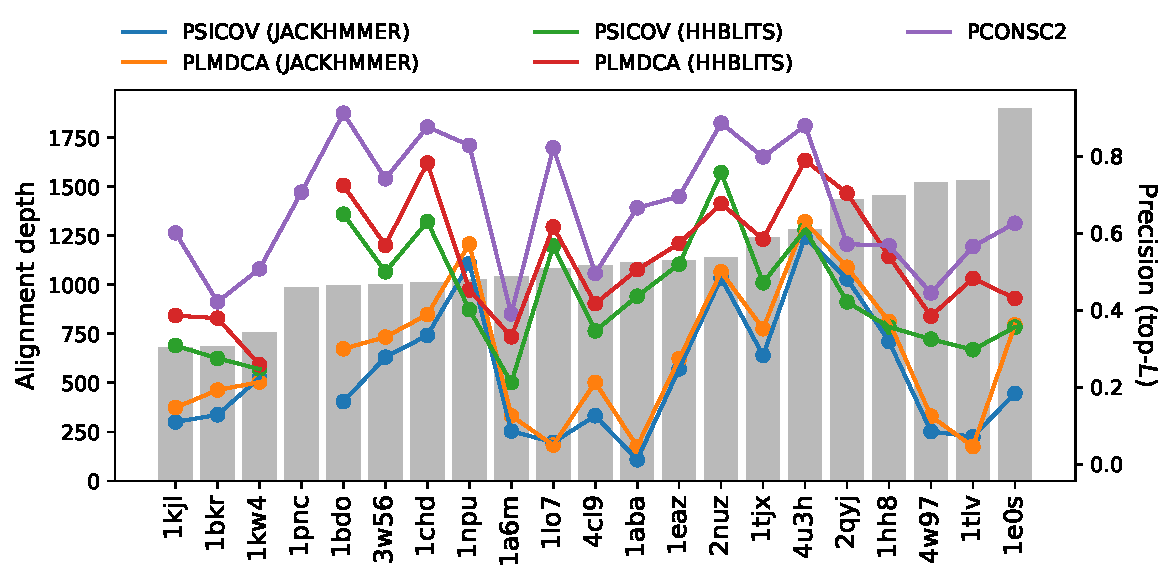
\includegraphics[width=\textwidth]{ample_proof_globpreccomp.pdf}
        \caption{}
        \label{fig:ample_proof_globpreccomp}
    \end{subfigure}
    
    \begin{subfigure}[b]{\textwidth}
        \centering
        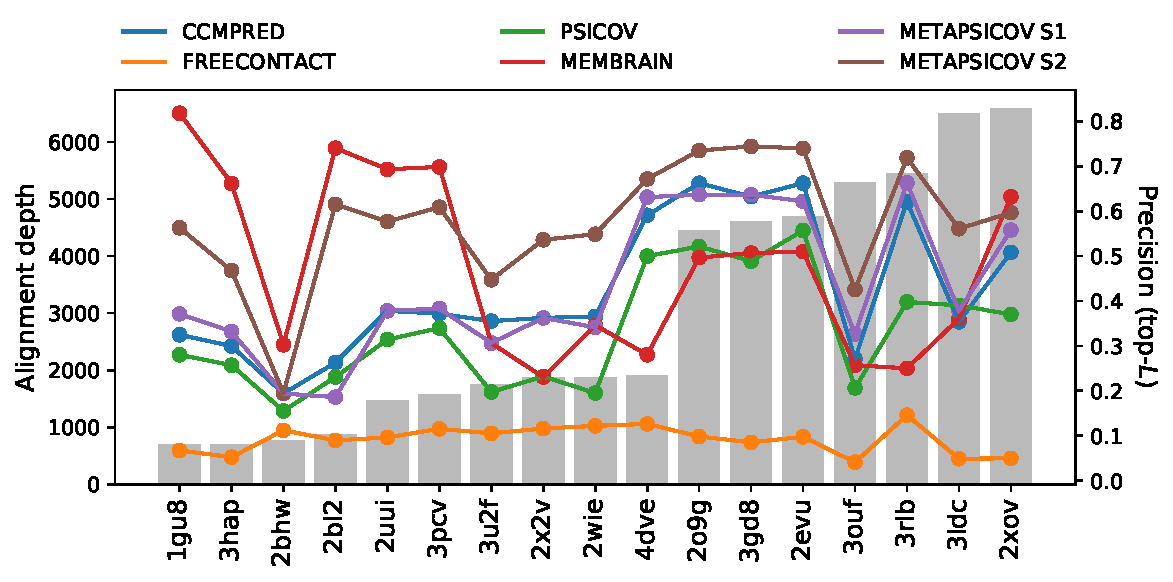
\includegraphics[width=\textwidth]{ample_proof_tmpreccomp.pdf}
        \caption{}
        \label{fig:ample_proof_tmpreccomp}
    \end{subfigure}
    
    \caption[Alignment depth and contact precision analysis of globular and transmembrane protein targets]{Alignment depth and contact precision analysis of (a) globular and (b) transmembrane protein targets. Contact predictions were obtained with four different contact prediction algorithms. Precision scores were calculated for the top-$L$ contact pairs. For illustrative purposes the marker size has been altered to indicate target chain length.}
    \label{fig:ample_proof_preccomp}
\end{figure}

The precision of coevolution-based contact prediction depends on alignment depth. However, results in this study suggest that alignment depth is not exclusively the key to precise contact prediction. The data shows that four targets have precision values for top-$L$ contact pairs of less than 50\% correctly predicted contact pairs whilst six targets contain at least 80\% (\cref{fig:ample_proof_globpreccomp}). This contrasts transmembrane protein targets where eleven CCMPRED and METAPSICOV STAGE1 top-$L$ contact pairs contain less than 50\% correct predictions whilst no set contains more than 80\% correct ones (\cref{fig:ample_proof_tmpreccomp}). MEMBRAIN predictions are slightly more precise, with a single set containing more than 80\% and nine less than 50\% correct contact pairs (\cref{fig:ample_proof_tmpreccomp}). However, one noticable difference between MEMBRAIN and CCMPRED/METAPSICOV STAGE1 contact predictions is that the former performs much better for transmembrane protein targets with less than 2,000 effective sequences, whilst the latter perform better for most other targets (\cref{fig:ample_proof_tmpreccomp}).

CCMPRED is one of three raw contact predictions that METAPSICOV uses \cite{Jones2015-vq}. Thus, it is of interest to identify if the addition of the remaining two and the first stage filtering of the METAPSICOV algorithm results in more accurate contact predictions compared to CCMPRED. However, only in about half of the cases under investigation does METAPSICOV STAGE1 top-$L$ contact pairs outperform CCMPRED ones (\cref{fig:ample_proof_tmpreccomp}).

\subsection{Protein structure prediction}

\begin{figure}[H]
    \centering
    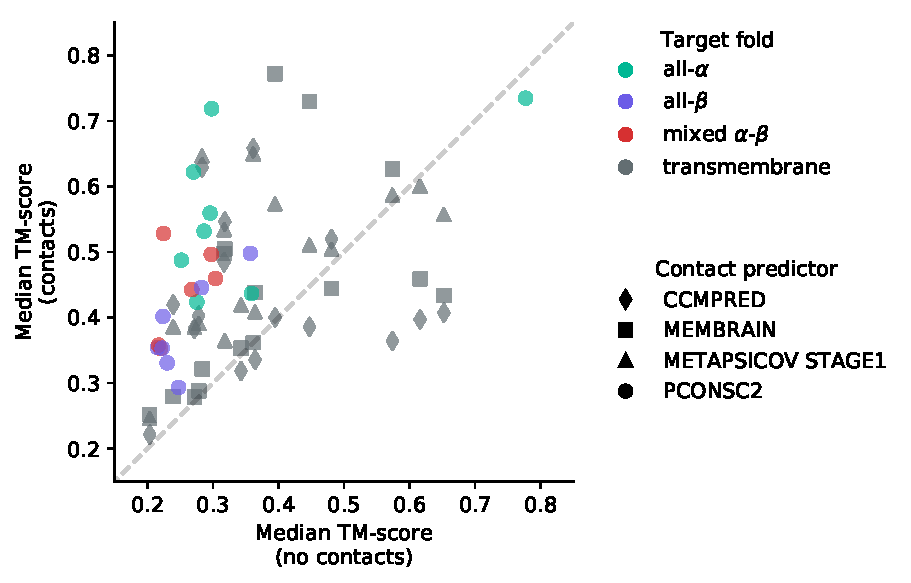
\includegraphics[width=\textwidth]{ample_proof_comproscon.pdf}
    \caption[Effect of contact distance restraints on \textit{ab initio} decoy quality]{Effect of contact distance restraints on \textit{ab initio} decoy quality by comparison of unrestrained (\textit{no contacts}) and contact-restrained (\textit{contacts}) median TM-scores for 1,000 decoys per target. Colours indicate the target fold and symbols the contact prediction algorithm.}
    \label{fig:ample_proof_comproscon}
\end{figure}

